\documentclass[border=0.8ex,svgnames,tikz,varwidth]{standalone}
\usepackage{amsmath,mathtools}
\usepackage{fontspec}
\setmainfont{Source Serif 4}
\setsansfont{Source Sans 3}
\setmonofont{Source Code Pro}
\usetikzlibrary{positioning,calc,fit,shapes,arrows.meta}
\begin{document}
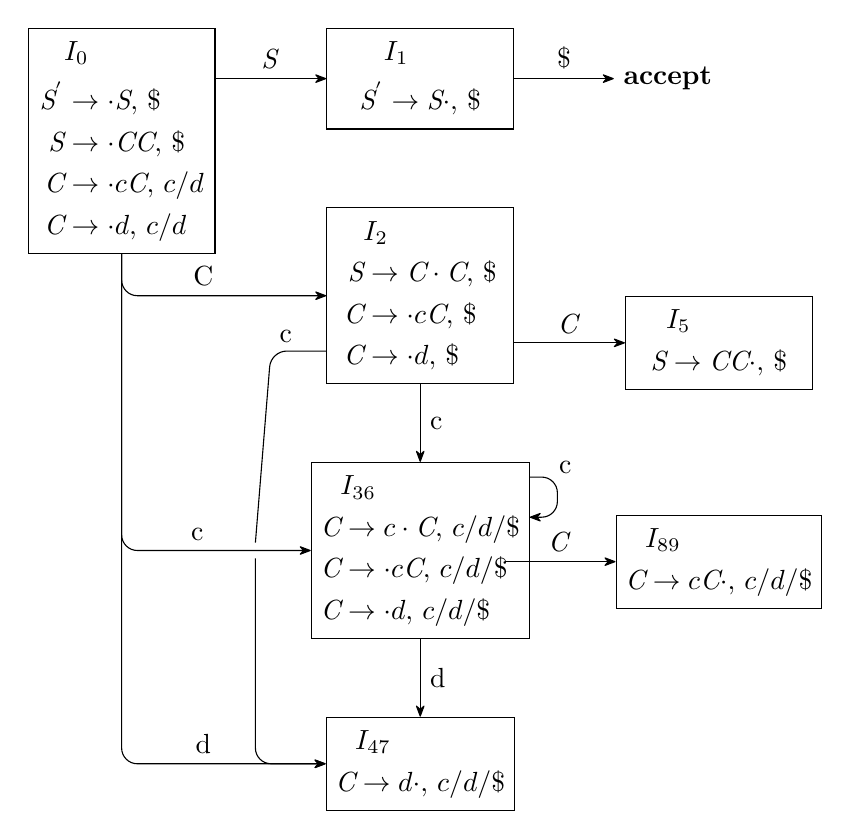
\begin{tikzpicture}
  \begin{scope}[
    every node/.style={
      rectangle,
      draw,
      minimum width=6.75em,
    },
    setanchor/.style={
      anchor=north west,
    },
    ]
    % I0
    \node (I0) at (0,0)
    {$\begin{aligned}
      & I_{0}\\
      \textit{S}^{'} &\rightarrow \cdot\textit{S},\,\$\\
      \textit{S} &\rightarrow \cdot\textit{C}\textit{C},\,\$\\
      \textit{C} &\rightarrow \cdot{}c\textit{C},\,c/d\\
      \textit{C} &\rightarrow \cdot{}d,\,c/d
    \end{aligned}$};

    % I1
    \node [right=4em of I0.north east,setanchor] (I1)
    {$\begin{aligned}
      & I_{1}\\
      \textit{S}^{'} &\rightarrow \textit{S}\cdot,\,\$
    \end{aligned}$};

    % I2
    \node [below=2.8em of I1] (I2)
    {$\begin{aligned}
      & I_{2}\\
      \textit{S} &\rightarrow \textit{C}\cdot\textit{C},\,\$\\
      \textit{C} &\rightarrow \cdot{}c\textit{C},\,\$\\
      \textit{C} &\rightarrow \cdot{}d,\,\$
    \end{aligned}$};

    % I36
    \node [below=2.8em of I2] (I36)
    {$\begin{aligned}
      & I_{36}\\
      \textit{C} &\rightarrow c\cdot\textit{C},\,c/d/\$\\
      \textit{C} &\rightarrow \cdot{}c\textit{C},\,c/d/\$\\
      \textit{C} &\rightarrow \cdot{}d,\,c/d/\$
    \end{aligned}$};

    % I47
    \node [below=2.8em of I36] (I47)
    {$\begin{aligned}
      & I_{47}\\
      \textit{C} &\rightarrow d\cdot,\,c/d/\$
    \end{aligned}$};

    % I5
    \node [right=4em of I2.east,setanchor] (I5)
    {$\begin{aligned}
      & I_{5}\\
      \textit{S} &\rightarrow \textit{C}\textit{C}\cdot,\,\$
    \end{aligned}$};

    % I89
    \node [below=4.5em of I5] (I89)
    {$\begin{aligned}
      & I_{89}\\
      \textit{C} &\rightarrow c\textit{C}\cdot,\,c/d/\$
    \end{aligned}$};
  \end{scope}
  \begin{scope}[
    myarrow/.style={
      ->,
      rounded corners=2mm,
      >=Stealth[round],
      % very thick,
    },
    ]
    \draw (I2.east) ++ (1.6em,0) coordinate (oI2);
    \draw (I2.west) ++ (0,-2em) coordinate (oI2west_start);
    \draw (I36.east) ++ (1.6em,0) coordinate (oI36);

    % Path I0
    \draw [myarrow] (I1.west) ++(-4em,0) -- node [above] {\textit{S}} ++(4em,0);
    \draw [myarrow] (I0) |- (I2);
    \draw [myarrow] (I0) |- (I36);
    \draw [myarrow] (I0) |- (I47);
    \node [above] at ($(I0.south |- I2.west)!0.4!(I2.west)$) {C};
    \node [above] at ($(I0.south |- I36.west)!0.4!(I36.west)$) {c};
    \node [above] at ($(I0.south |- I47.west)!0.4!(I47.west)$) {d};
    \node [label=left:c,below right=-1.25em] at (oI2west_start) {};

    % Path I1
    \draw [myarrow] (I1.east) -- node [above] {\(\$\)} ++(3.6em,0) node [right] {\textbf{accept}};

    % Path I2
    \draw [myarrow] (I2) -- node [right] {c} (I36);
    \draw (I36.west) ++(-2em,+0.1) coordinate (I36interruption1);
    \draw (I36.west) ++(-2em,-0.1) coordinate (I36interruption2);
    \draw [myarrow,-] (oI2west_start) -- ++(-2em,0) -- (I36interruption1);
    \draw [myarrow] (I36interruption2) |- (I47);
    \draw [myarrow] (I5.west) ++(-4em,0) -- node [above] {\textit{C}} ++(4em,0);

    % Path I36
    \draw (I36.north east) ++ (0,-0.55em) coordinate (oI3iI3start);
    \draw (I36.north east) ++ (0,-2em) coordinate (oI3iI3end);
    \draw [myarrow] (oI3iI3start) -- ++(1em,0) |- (oI3iI3end);
    \draw [myarrow] (I36) -- node [right] {d} (I47);
    \draw [myarrow] (I89.west) ++(-4em,0) -- node [above] {\textit{C}} ++(4em,0);
    \node [label=right:c,below left=-1em] at (oI3iI3start) {};
  \end{scope}
\end{tikzpicture}
\end{document}
